\documentclass[12pt]{article}

\usepackage[vmargin=0.75in, left=0.75in, right=0.75in,  
				headheight=0.75in, headsep=12pt]{geometry}
\usepackage{multirow}
\usepackage{graphicx}
\usepackage{float}
\usepackage{amsmath}
\usepackage{fancyhdr}
\usepackage[parfill]{parskip}
\usepackage{bm}

\bibliographystyle{apa}
\setlength\bibindent{2em}
\usepackage[square,numbers,comma, sort & compress]{natbib}
\makeatletter
\renewcommand\NAT@bibsetnum[1]{\settowidth\labelwidth{\@biblabel{#1}}%
   \setlength{\leftmargin}{\bibindent}\addtolength{\leftmargin}{\dimexpr\labelwidth+\labelsep\relax}%
   \setlength{\itemindent}{-\bibindent}%
   \setlength{\listparindent}{\itemindent}
\setlength{\itemsep}{\bibsep}\setlength{\parsep}{\z@}%
   \ifNAT@openbib
     \addtolength{\leftmargin}{\bibindent}%
     \setlength{\itemindent}{-\bibindent}%
     \setlength{\listparindent}{\itemindent}%
     \setlength{\parsep}{0pt}%
   \fi
}
\makeatother

\usepackage{array}
\newcolumntype{x}[1]{>{\centering\arraybackslash\hspace{0pt}}p{#1}}
\newcolumntype{y}[1]{>{\raggedright\arraybackslash\hspace{0pt}}p{#1}}
\newcolumntype{z}[1]{>{\raggedleft\arraybackslash\hspace{0pt}}p{#1}}
\newcolumntype{+}{>{\global\let\currentrowstyle\relax}}
\newcolumntype{^}{>{\currentrowstyle}}
\newcommand{\rowstyle}[1]{\gdef\currentrowstyle{#1}%
	#1\ignorespaces
}

\title{%
	OpenFOAM ABL Experiment \texttt{\#}1\\
}

\date{%
	03/23/2017
}

\author{%
	Matthew W. McKenna\\
	B.S.M.E., Wichita State University, 2013
}

\begin{document}
%\setlength{\parindent}{0pt}
%\setlength{\parskip}{\baselineskip}
\maketitle
\thispagestyle{empty}
\pagebreak
\section{Objective}
A precursor simulation of the turbulent atmospheric boundary layer (ABL) is necessary for developing a turbulent inlet boundary condition within more complex flow domains which would otherwise conflict with cyclic (periodic) boundary conditions.  The purpose of this experiment is to produce a neutrally stable, turbulent ABL that will serve this purpose.

\section{Boundary Conditions}
This report includes results and analysis for simulations which build off of a base case where turbulence has developed with bulk velocity ($\bar{U}$) of 3 m/s and kinematic viscosity ($\nu$) of $1.55 \times 10^{-5}$ m$^2$/s.  Turbulence is maintained using \texttt{meanVelocityForce} within \texttt{OpenFOAM}'s \texttt{fvOptions}, which calculates the required forcing term of the Navier-Stokes equation in order to maintain the bulk velocity.

The domain is $1250 \text{m} \times 800 \text{m} \times 800 \text{m}$ in the $x$, $y$, and $z$ directions, respecively, in which $x$ is the streamwise direction and $y$ is the vertical direction.  This is discretized into a mesh of 125 $\times$ 200 $\times$ 80 cells, where the cell dimensions in the horizontal directions are constant at 10 m.  Cell dimensions in the vertical direction varies using a geometric expansion with an overall expansion ratio ($\delta_n/\delta_0$) of 10, resulting in 1.02 m cell height at the bottom and 10.2 m at the top.

Each simulation was run for 5000 seconds, which is approximately 10 flow-through times.  Velocity probes at the domain center point ($x=625$, $y=400$, $z=400$) and along the vertical line passing through the domain center were recorded at 10 Hz, resulting in 50,000 vector values for each point.  However, only the last 1000 seconds (10,000 values) are used for analysis.

All simulations were run using the following boundary conditions:
\begin{itemize}
	\item Domain
	\footnote{Symmetric and cyclic boundary conditions are derived boundary conditions and cannot have further constraints imposed upon them.}
	\begin{table}[H]
	%\centering
	\begin{tabular}{+z{3cm} ^y{8cm}}
		Top: & Symmetric (\texttt{symmetryPlane}) \\
		Sides: & Symmetric (\texttt{symmetryPlane}) \\
		Inlet: & Cyclic/Periodic (\texttt{cyclic}) \\
		Outlet: & Cyclic/Periodic (\texttt{cyclic}) \\
		Bottom: & No-slip (\texttt{wall}) \\
	\end{tabular}
	\end{table}
	%
	\item Velocity (\texttt{U})
	\begin{table}[H]
	%\centering
	\begin{tabular}{+z{3cm} ^y{8cm}}
		Bottom: & \texttt{fixedValue, uniform(0,0,0)} \\
	\end{tabular}
	\end{table}
	%	
	\item Pressure (\texttt{p})
	\begin{table}[H]
	%\centering
	\begin{tabular}{+z{3cm} ^y{8cm}}
		Bottom: & \texttt{fixedValue; uniform 0;} \\
	\end{tabular}
	\end{table}
	%
	\item Turbulent Viscosity (\texttt{nut})
	\begin{table}[H]
	%\centering
	\begin{tabular}{+z{3cm} ^y{8cm}}
		Bottom: & \textit{(varied with desired wall-conditioning)}
	\end{tabular}
	\end{table}
	%
	\item Turbulent Kinetic Energy (\texttt{k}) 
	\begin{table}[H]
	%\centering
	\begin{tabular}{+z{3cm} ^y{8cm}}
		Bottom: & \texttt{fixedValue; uniform 0;} \footnotemark
	\end{tabular}
	\end{table}
\end{itemize}
	\footnotetext{De Villers \citep{devillers01} has suggested that TKE is not approximated well by this boundary condition for $y^+>20$.  The \texttt{zeroGradient} boundary condition is suggested instead.} 

\section{Simulations}
\subsection{Determination of Stability}
Before further analysis can be conducted, the flow must be allowed to become statistically stable.  Until a more robust method has been established, two methods are currently being utilized.  The first is assumption based off visual assessment of the instantaneous fluctuations at the domain center.  The second, which has only recently been implemented, is assessment of the auto-covariance of a fluctuating velocity component with increasing time lag \cite{shi01, wyngaard01}.  Here, the mean product of two fluctuating components at the same point, but different times, or auto-covariance:
\begin{equation}
	R_{uu}(\tau) = \frac{1}{T} \int_0^T u'(t)u'(t+\tau)dt	
\end{equation}
At zero time lag ($\tau=0$), the auto-covariance becomes the variance $R_{uu}(0)=\sigma_u^2$.  The auto-correlation is the auto-covariance normalized by the variance:
\begin{equation}
C_{uu} = \frac{R_{uu}}{\sigma_u^2}
\end{equation}
The auto-covariance should tend toward zero as the time lag increases \citep{shi01}, indicating less correlation with itself at the reference time.

\subsection{Evaluating Near-Wall Behavior}
Each simulation was probed at a rate of 10 Hz at every cell center along a line at the domain center.  The last 10,000 values of the streamwise component at every point was averaged to produce a mean vertical velocity profile.  This profile was fed into a curve-fitting algorithm to produce coefficient values for the function
\begin{equation}
A \frac{y u^*}{\nu} + B
\end{equation}
which minimize the sum of square errors between the points and the line.  Here, $A$ and $B$ are the coefficients being solved for, $u^*$ is the friction velocity, and $\nu$ is the kinematic viscosity used in the simulation.  However, due to a large $y^+$ compared to DNS simulations, it was not known whether an appropriate friction velocity could be found using the Newtonian laminar shear stress model:
\begin{align}
\tau_w &= \left. \mu \frac{\partial u}{\partial y} \right|_{y=0} \\
u^* &= \sqrt{\frac{\tau_w}{\rho}} 
\end{align}
Instead, the value of $u^*$ was initialized at a best-guess value and incremented until the covariance between the data and the curve-fit line had reached an acceptable minimum threshhold.  The final covariances are listed along with the other results for each simulation.  As an additional metric for how well the equation fits the data, the $R^2$ value is also listed.

\subsection{Without Wall Contitioning}
The first simulations were run without the use of wall conditioning (i.e. wall functions).  The bottom boundary condition for the turbulent viscosity ($\nu_\tau$) is \texttt{zeroGradient}, rather than specifying a value and wall function.  The sub-grid scale (SGS) models used were the Smagorinsky and One-Equation Eddy Viscosity models.

Figures \ref{none_keq_stab} and \ref{none_sm_stab} seem to be stable based off the trend of instantaneous component fluctuations.  However, while auto-correlation of the spanwise and vertical components trend toward 0, the streamwise component remains nearly constant at 1, indicating very strong correlation.  This result is disconcerting and is being investigated.  This is an indication of a mistake in the auto-correlation computation or in the simulation itself.

Figure \ref{none_keq_sm_log} shows the result of fitting the mean vertical velocity profiles to a linear function.  Both SGS models resulted in very similar curve fit equations, but did not match the theoretical linear model.  The One-Equation Eddy Viscosity model resulted in $u^* = 0.184$ m/s, $1/\kappa = 2.450 \pm 0.025$, and $B = -21.284 \pm 0.365$.  The Smagorinsky model resulted in $u^* = 0.186$ m/s, $1/\kappa = 2.455 \pm 0.024$, and $B = -21.599 \pm 0.343$.

\begin{figure}[H]
\centering
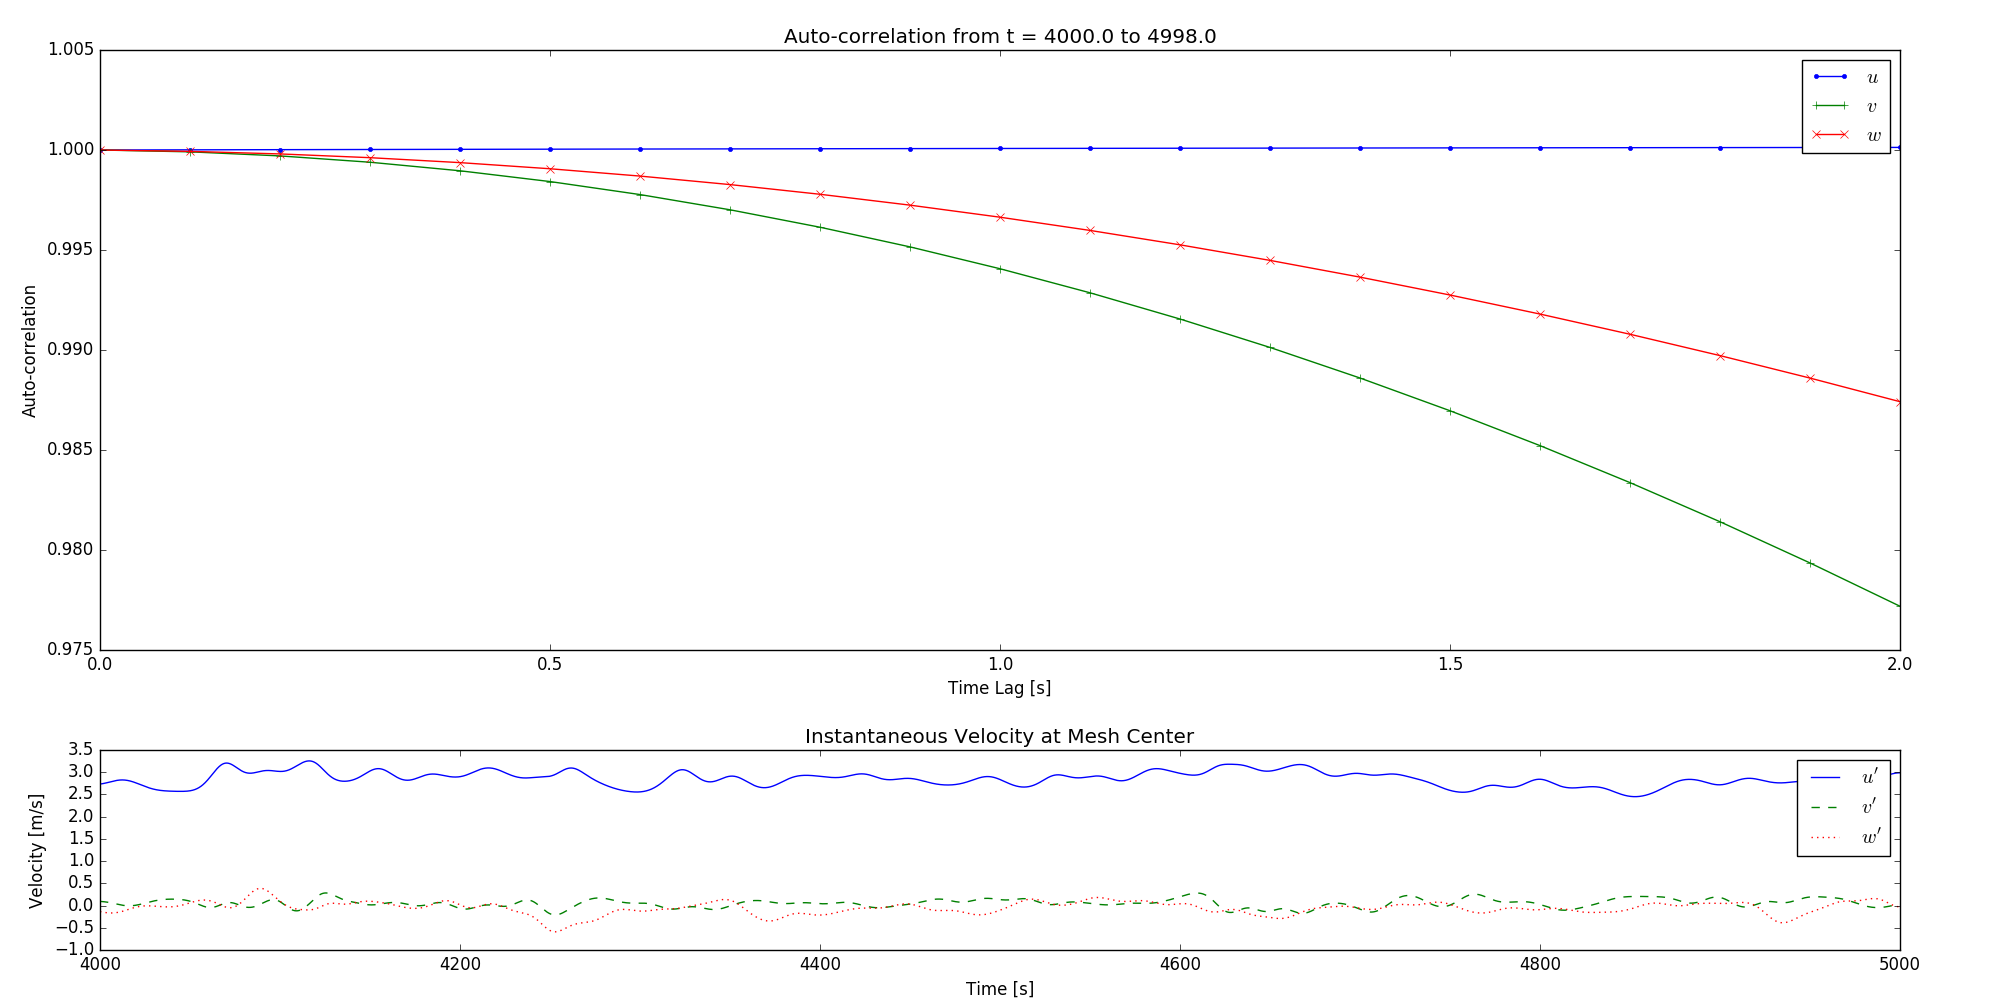
\includegraphics[scale=0.35]{none/keq_stability.png}
\caption{Auto-correlation of each velocity component with increased time lag (above) and instantaneous values of velocity components (below) for the One-Equation Eddy Viscosity SGS, with no wall conditioning.}
\label{none_keq_stab}
\end{figure}
  
\begin{figure}[H]
\centering
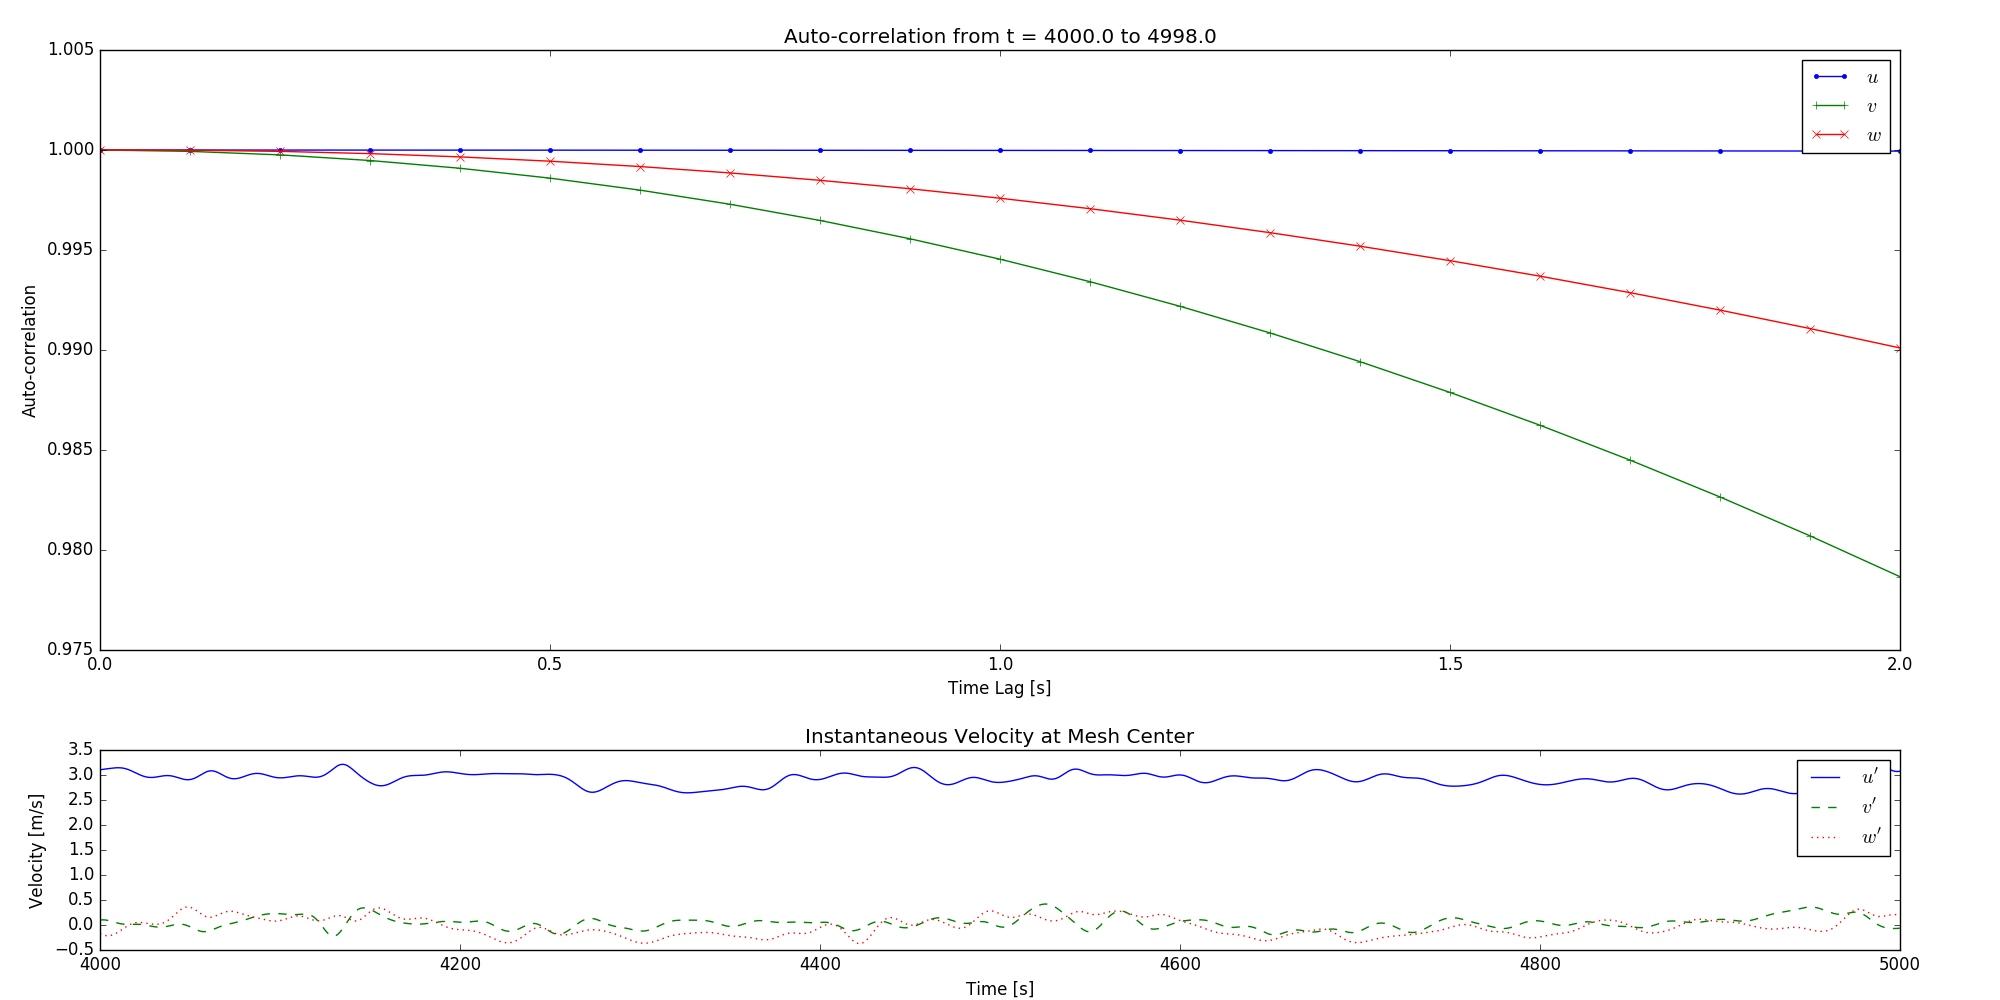
\includegraphics[scale=0.35]{none/sm_stability.png}
\caption{Auto-correlation of each velocity component with increased time lag (above) and instantaneous values of velocity components (below) for the Smagorinsky SGS, with no wall conditioning.}
\label{none_sm_stab}
\end{figure}

\begin{figure}[H]
\centering
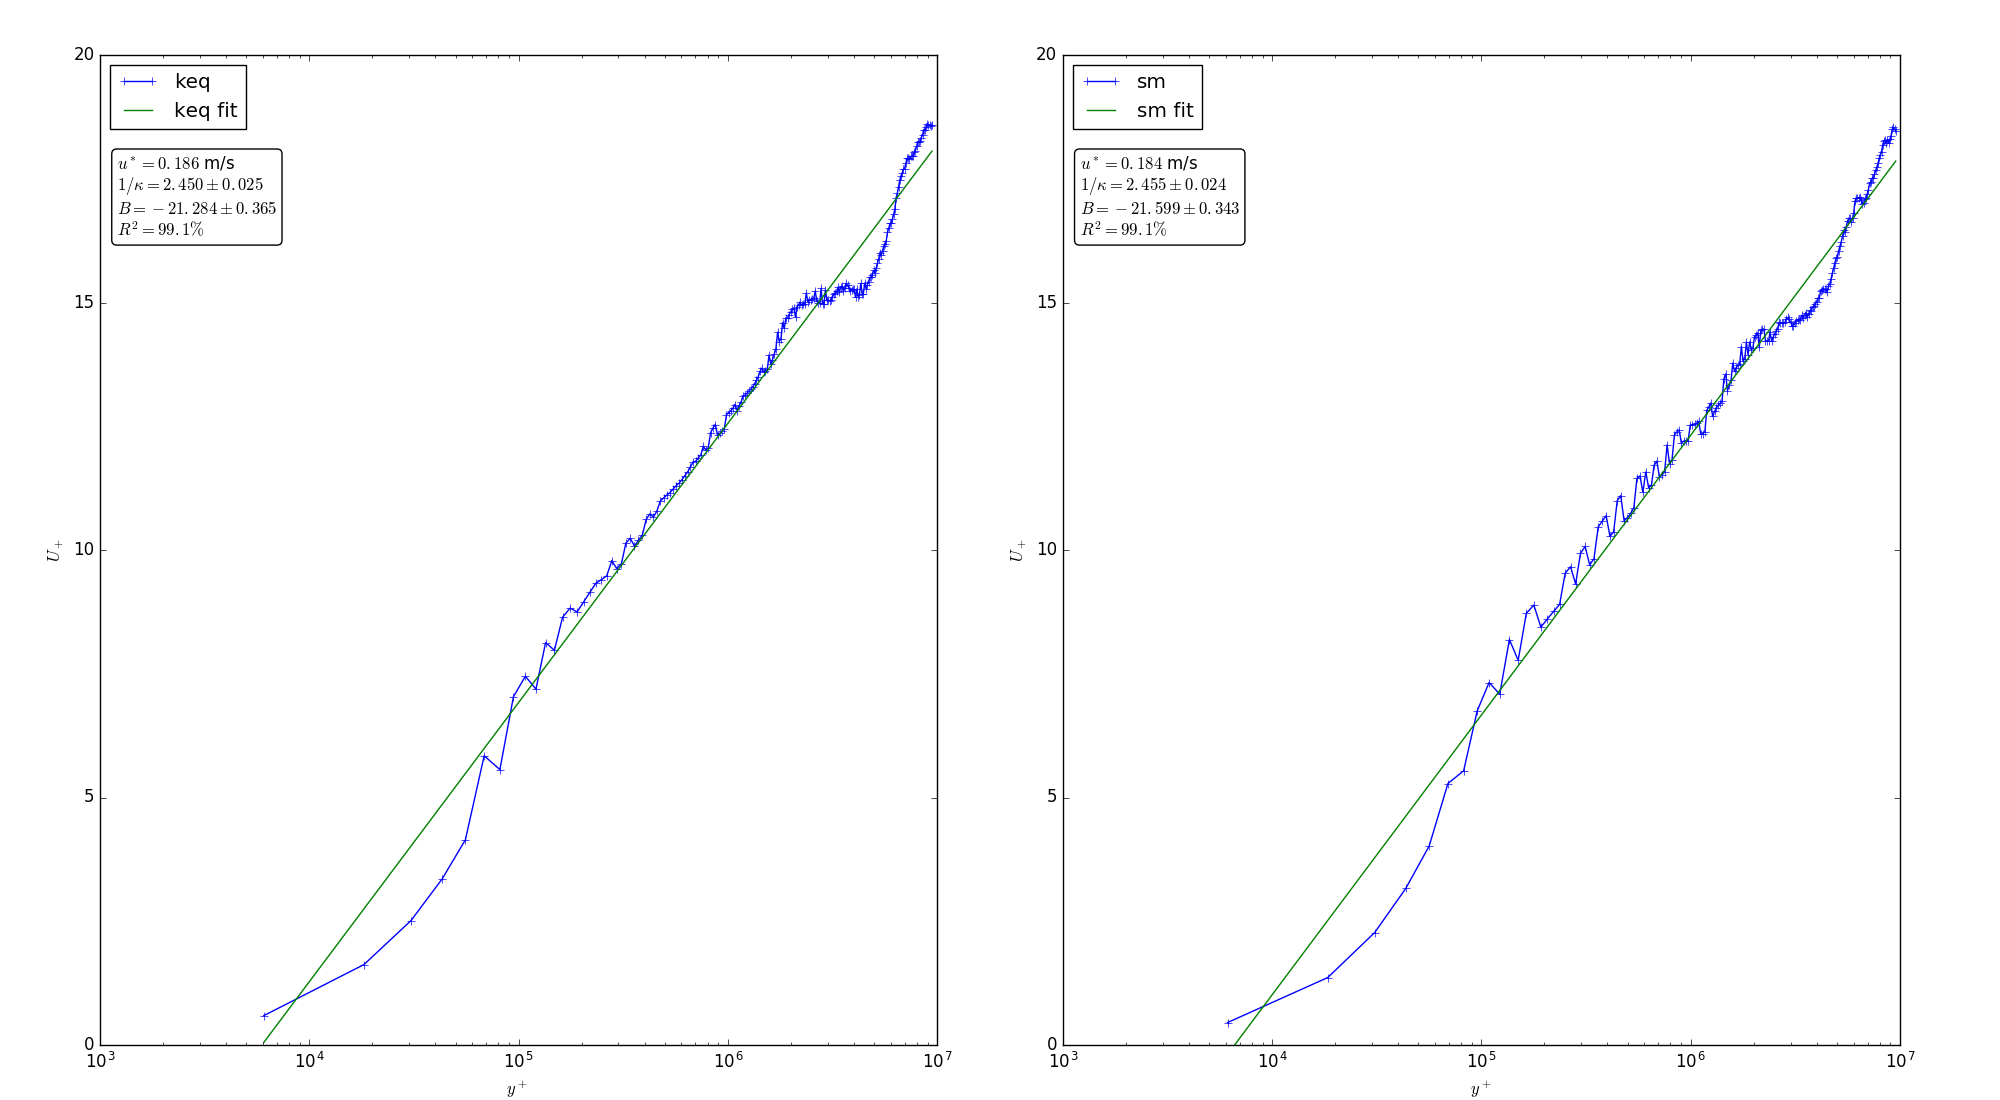
\includegraphics[scale=0.35]{none/keq_sm_log.png}
\caption{Log-linear fit of the mean vertical velocity profile for the One-Equation Eddy Viscosity (left) and the Smagorinsky (right) SGS models, without wall conditioning.}
\label{none_keq_sm_log}
\end{figure}

\subsection{\texttt{nutkWallFunction}}
This set of simulations were run with the \texttt{nutkWallFunction}, which is a near-wall SGS model that uses the TKE values at the surface to produce log-linear results.  The bottom boundary condition for the turbulent viscosity is where the \texttt{nutkWallFunction} usage is specified, along with the specification \texttt{fixedValue} at \texttt{uniform 1.55e-5}.  Once again, Smagorinsky and One-Equation Eddy Viscosity models were used as the primary SGS models.

Figures \ref{nutk_keq_stab} and \ref{nutk_sm_stab} seem to be stable based off the trend of instantaneous component fluctuations and show very similar auto-correlation results as the simulations without wall conditioning. 

Figure \ref{nutk_keq_sm_log} shows the result of fitting the mean vertical velocity profiles to a linear function.  Both SGS models resulted in very similar curve fit equations, but did not match the theoretical linear model.  The One-Equation Eddy Viscosity model resulted in $u^* = 0.142$, $1/\kappa = 2.450 \pm 0.038$, and $B = -16.225 \pm 0.543$.  The Smagorinsky model resulted in $u^* = 0.154$, $1/\kappa = 2.458 \pm 0.031$, and $B = -18.024 \pm 0.446$.

\begin{figure}[H]
\centering
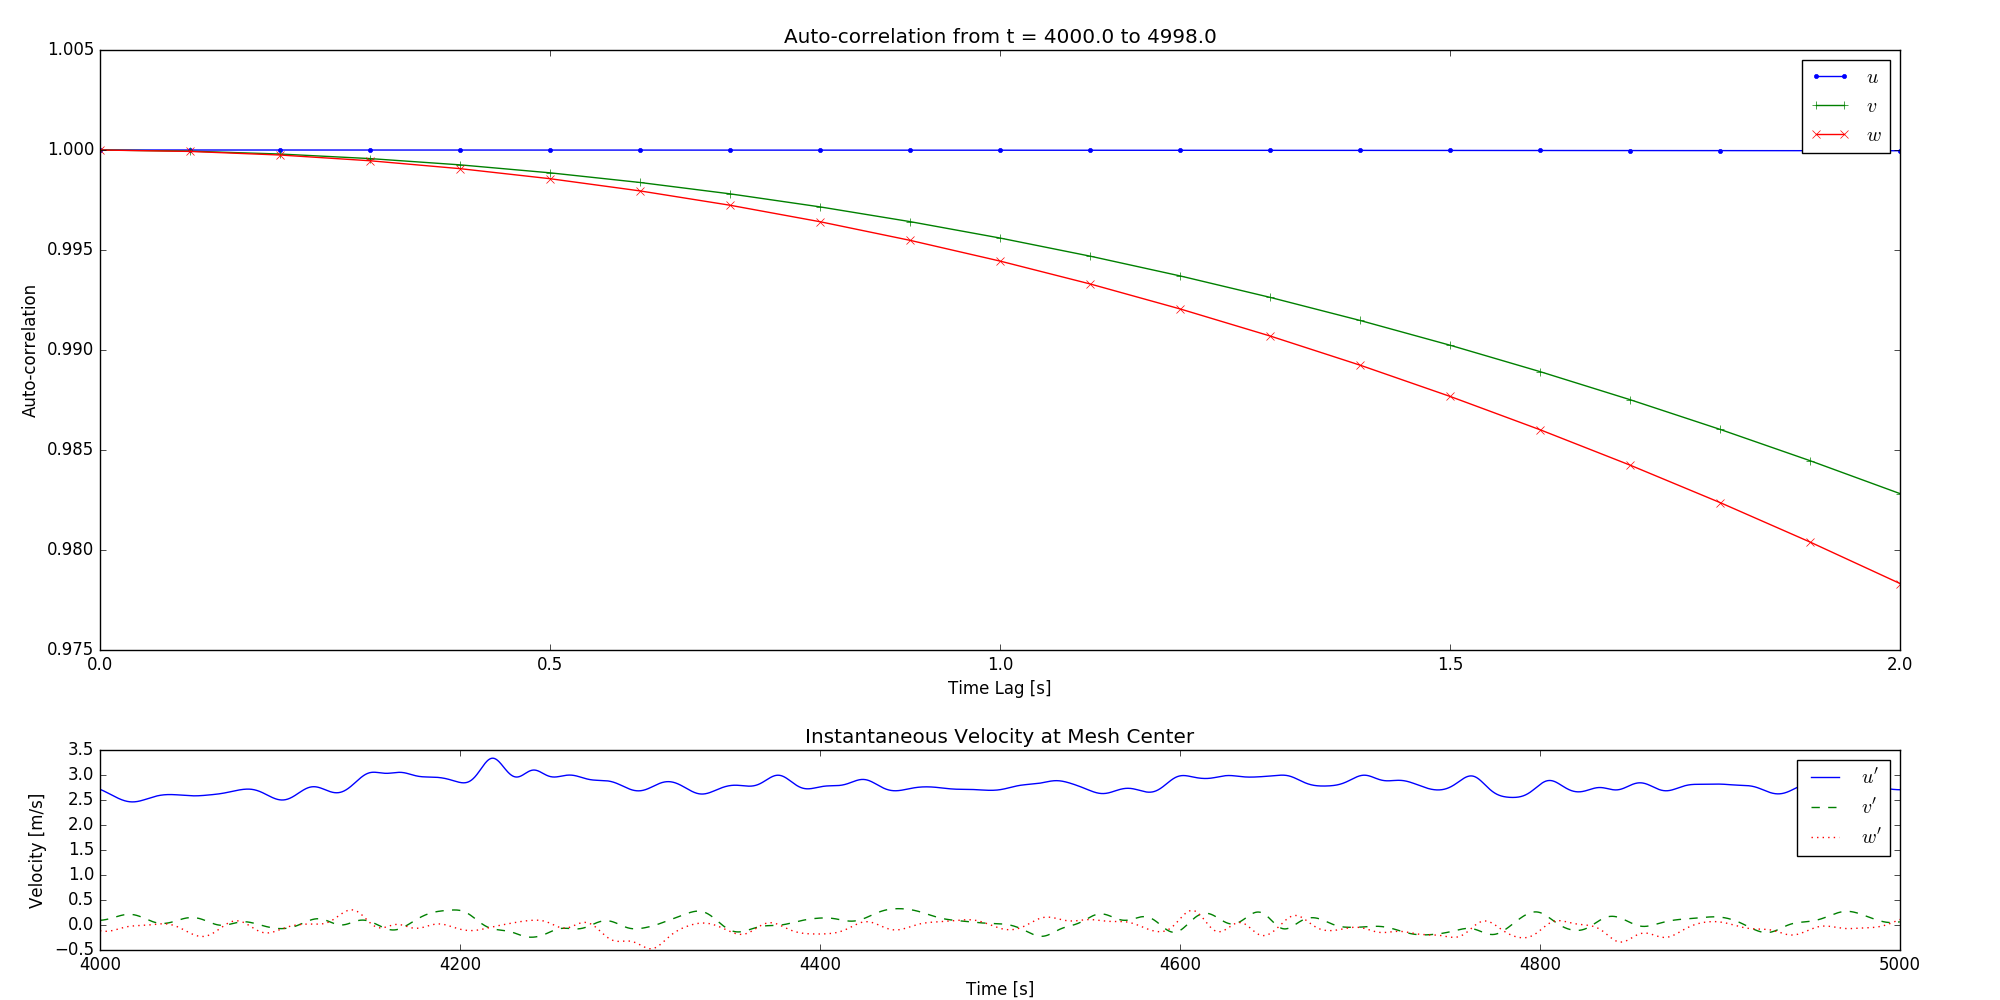
\includegraphics[scale=0.35]{nutk/keq_stability.png}
\caption{Auto-correlation of each velocity component with increased time lag (above) and instantaneous values of velocity components (below) for the One-Equation Eddy Viscosity SGS, using the \texttt{nutkWallFunction}.}
\label{nutk_keq_stab}
\end{figure}
  
\begin{figure}[H]
\centering
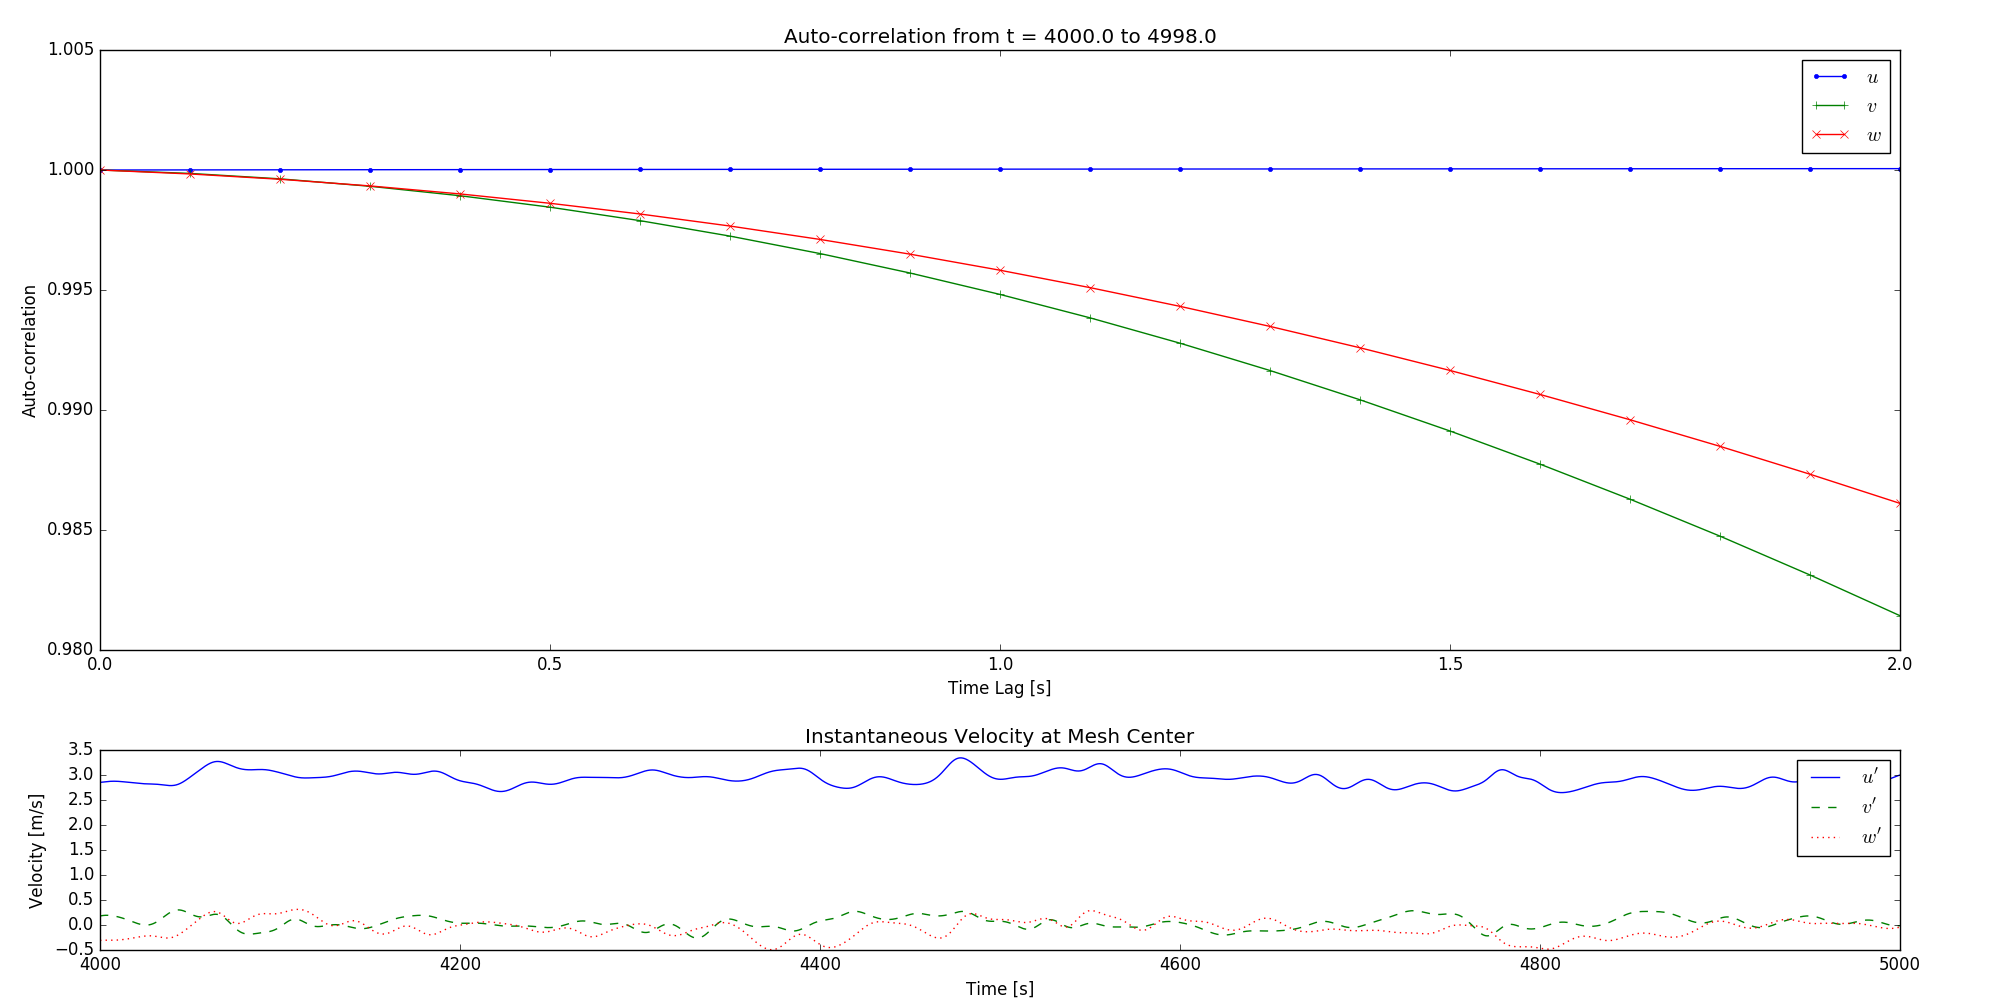
\includegraphics[scale=0.35]{nutk/sm_stability.png}
\caption{Auto-correlation of each velocity component with increased time lag (above) and instantaneous values of velocity components (below) for the Smagorinsky SGS, using the \texttt{nutkWallFunction}.}
\label{nutk_sm_stab}
\end{figure}

\begin{figure}[H]
\centering
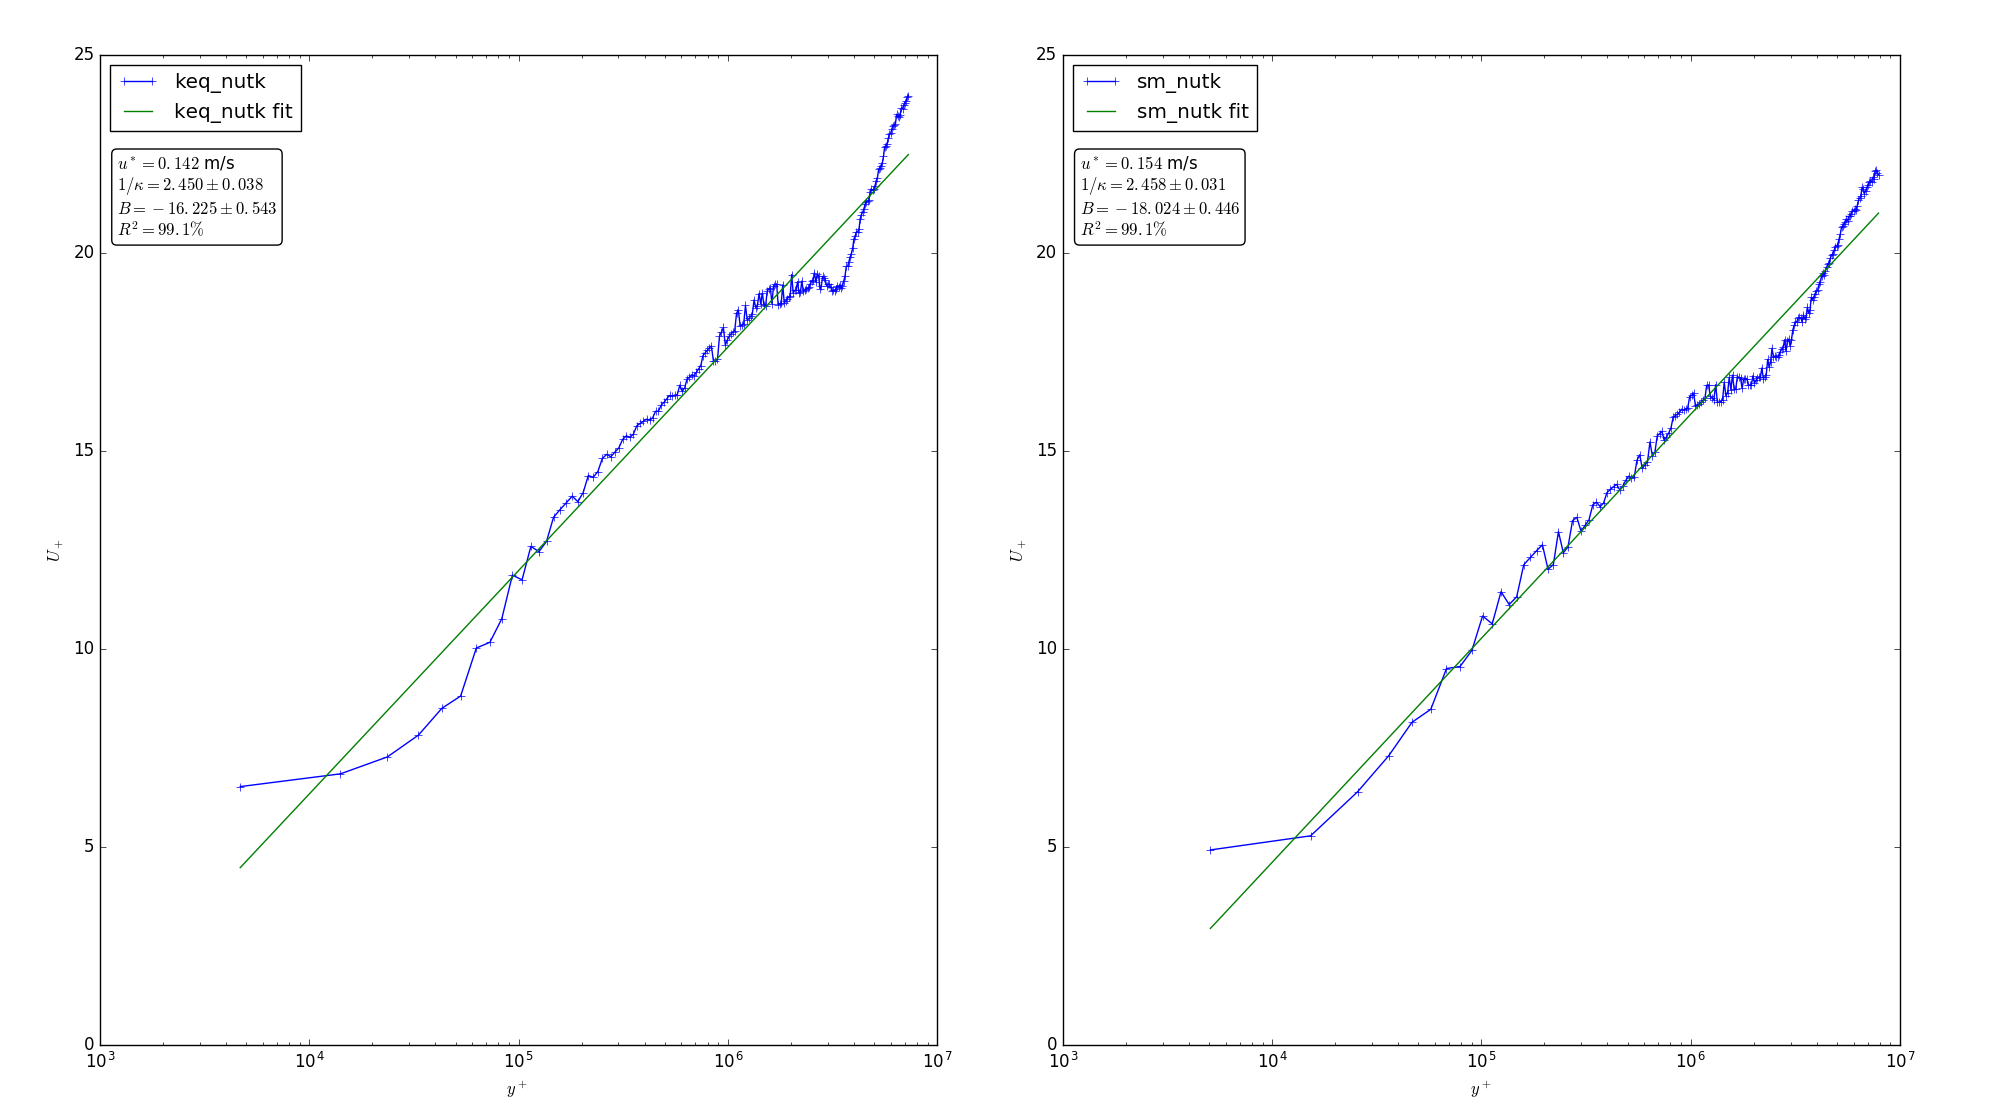
\includegraphics[scale=0.35]{nutk/keq_sm_log.png}
\caption{Log-linear fit of the mean vertical velocity profile for the One-Equation Eddy Viscosity (left) and the Smagorinsky (right) SGS models, using the \texttt{nutkWallFunction}.}
\label{nutk_keq_sm_log}
\end{figure}

\subsection{\texttt{nutkWallFunction} with Van Driest Dampening}
%This set of simulations were run with the \texttt{nutkWallFunction}, which is a near-wall SGS model that uses the TKE values at the surface to produce log-linear results.  The bottom boundary condition for the turbulent viscosity is where the \texttt{nutkWallFunction} usage is specified, along with the specification \texttt{fixedValue} at \texttt{uniform 1.55e-5}.  Once again, Smagorinsky and One-Equation Eddy Viscosity models were used as the primary SGS models.

Figures \ref{vd_nutk_keq_stab} and \ref{vd_nutk_sm_stab} seem to be stable based off the trend of instantaneous component fluctuations and show very similar auto-correlation results as the simulations without wall conditioning. 

Figure \ref{vd_nutk_keq_sm_log} shows the result of fitting the mean vertical velocity profiles to a linear function.  Both SGS models resulted in very similar curve fit equations, but did not match the theoretical linear model.  The One-Equation Eddy Viscosity model resulted in $u^* = 0.133$, $1/\kappa = 2.460 \pm 0.039$, and $B = -14.862 \pm 0.545$.  The Smagorinsky model resulted in $u^* = 0.139$ m/s, $1/\kappa = 2.452 \pm 0.029$, and $B = -15.686 \pm 0.403$.

\begin{figure}[H]
\centering
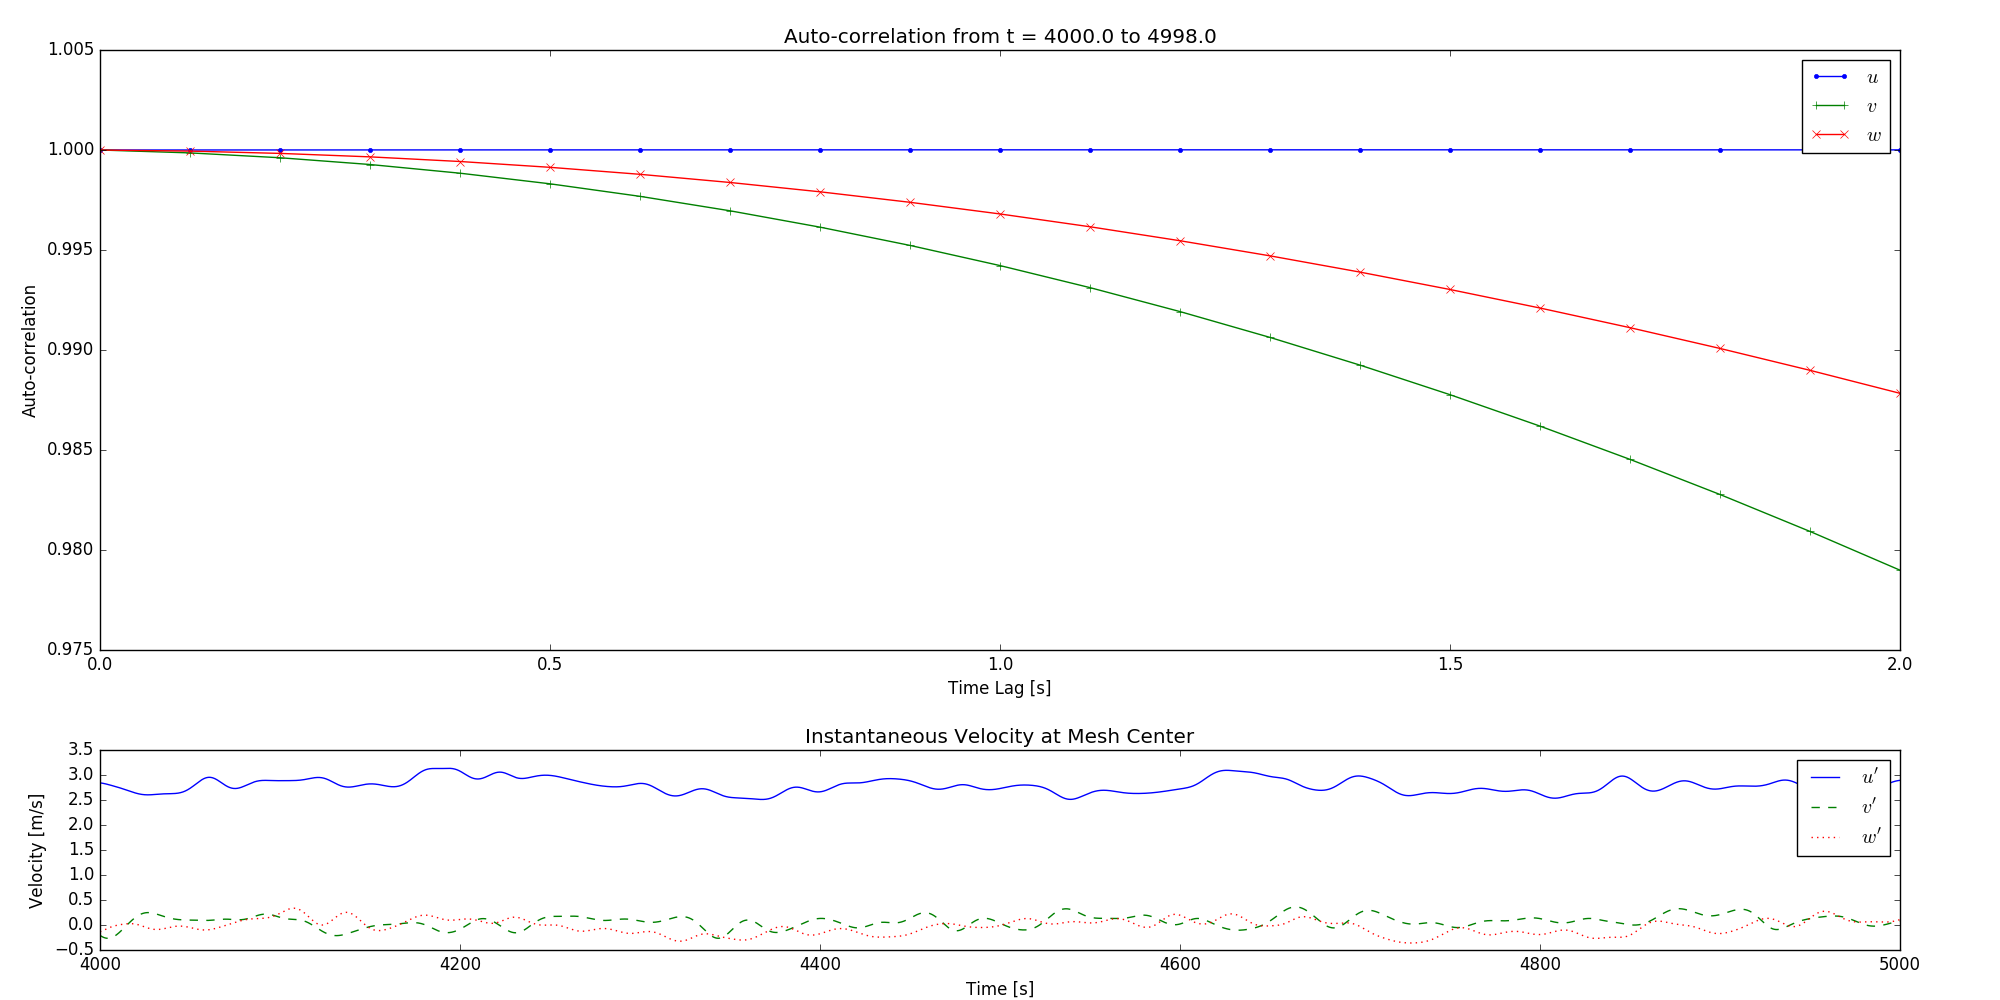
\includegraphics[scale=0.35]{vd_nutk/keq_stability.png}
\caption{Auto-correlation of each velocity component with increased time lag (above) and instantaneous values of velocity components (below) for the One-Equation Eddy Viscosity SGS, using the \texttt{nutkWallFunction} and Van Driest damping.}
\label{vd_nutk_keq_stab}
\end{figure}
  
\begin{figure}[H]
\centering
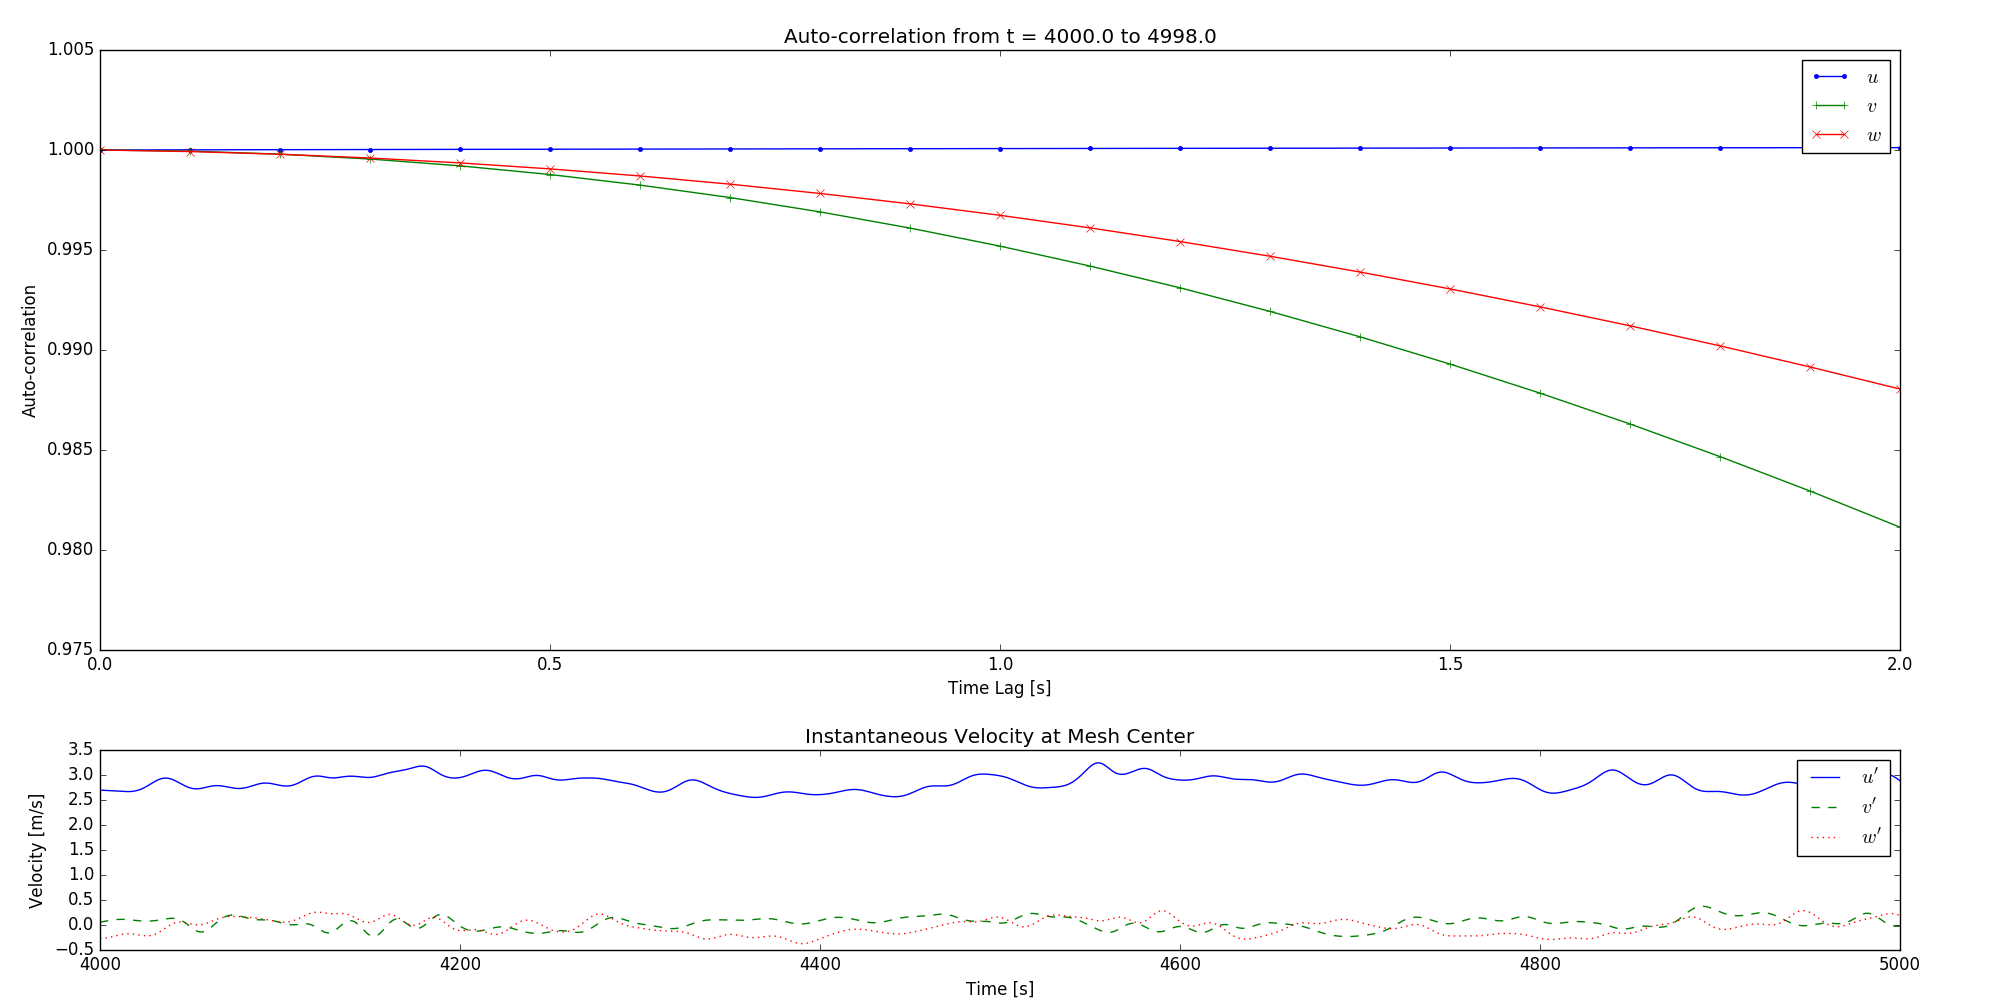
\includegraphics[scale=0.35]{vd_nutk/sm_stability.png}
\caption{Auto-correlation of each velocity component with increased time lag (above) and instantaneous values of velocity components (below) for the Smagorinsky SGS, using the \texttt{nutkWallFunction} and Van Driest damping.}
\label{vd_nutk_sm_stab}
\end{figure}

\begin{figure}[H]
\centering
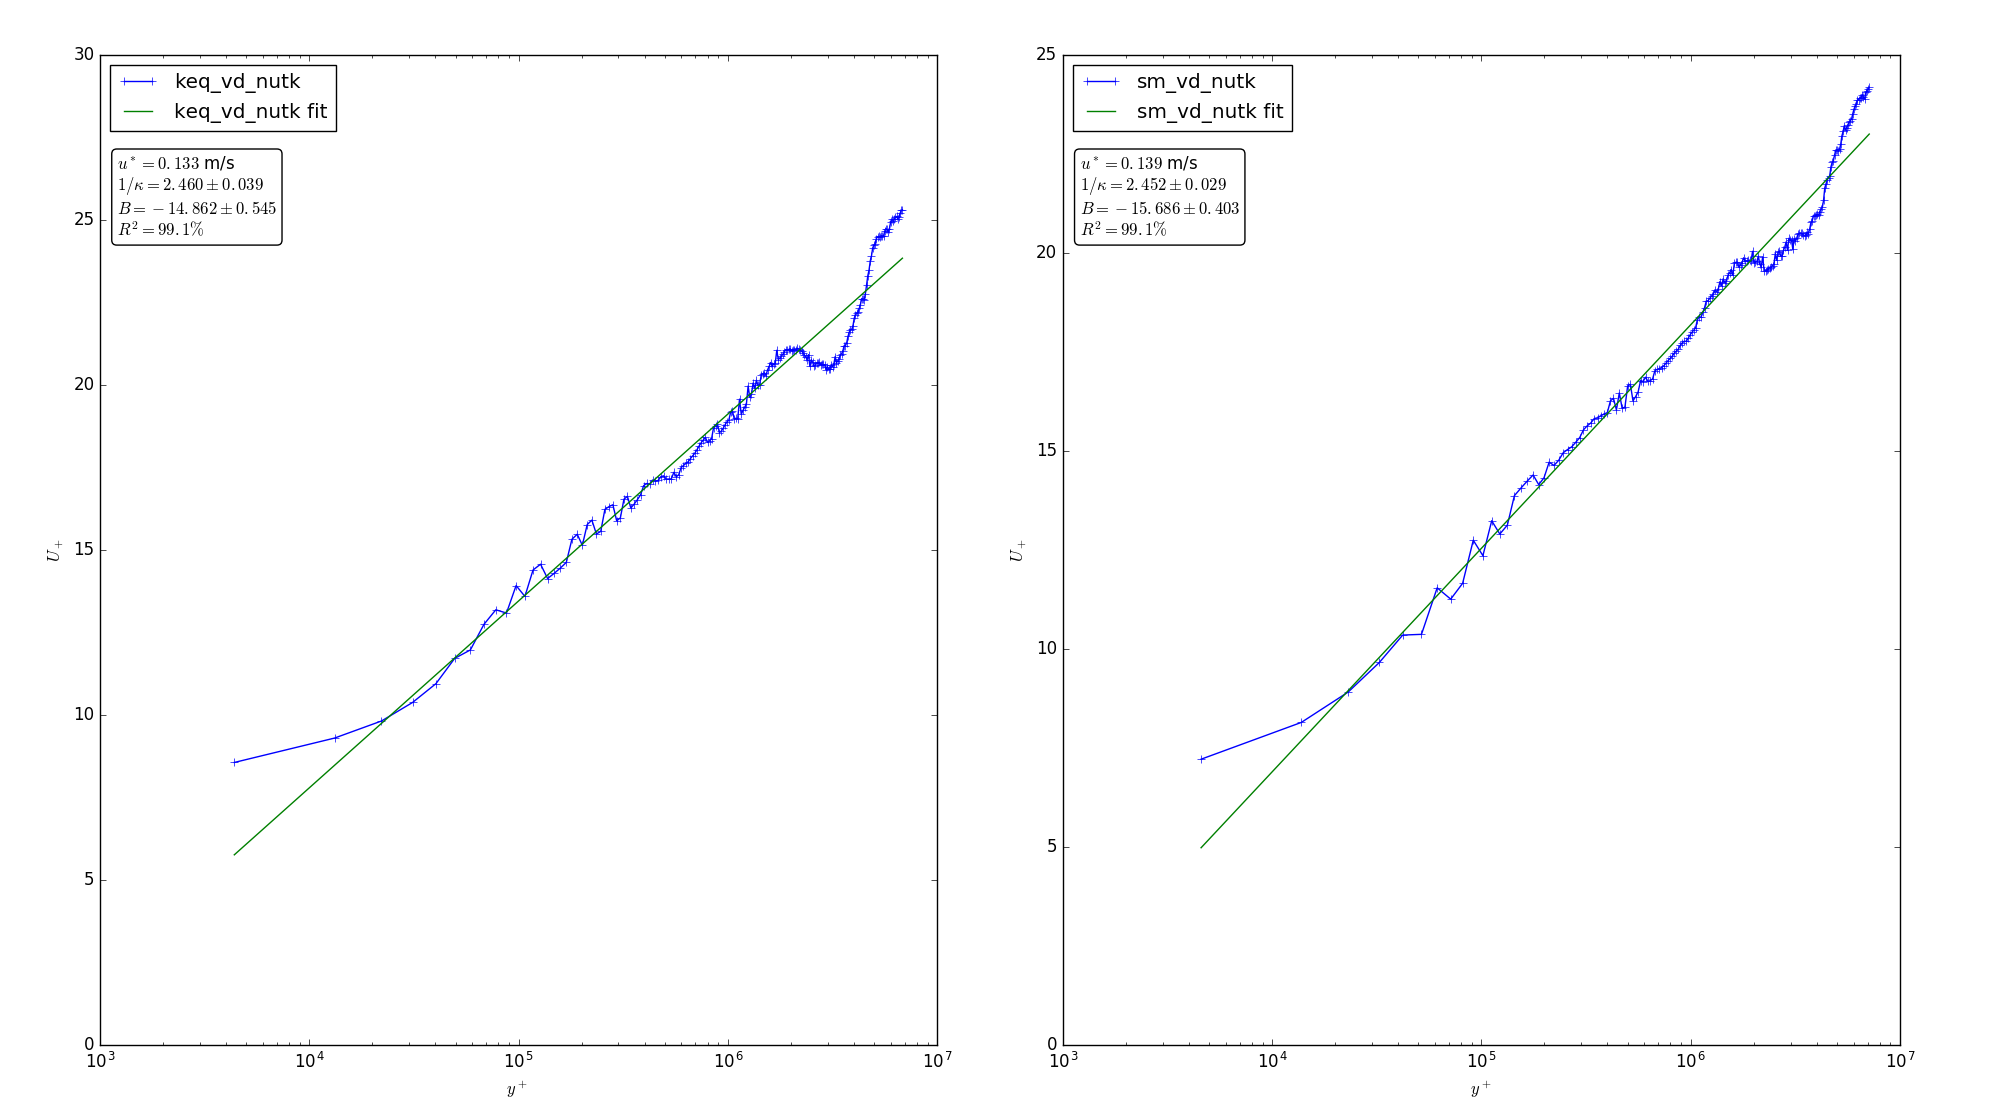
\includegraphics[scale=0.35]{vd_nutk/keq_sm_log.png}
\caption{Log-linear fit of the mean vertical velocity profile for the One-Equation Eddy Viscosity (left) and the Smagorinsky (right) SGS models, using the \texttt{nutkWallFunction} and Van Driest damping.}
\label{vd_nutk_keq_sm_log}
\end{figure}

\subsection{\texttt{nutUWallFunction}}
This set of simulations were run with the \texttt{nutUWallFunction}, which is a near-wall SGS model that uses the velocity values at the surface to produce log-linear results.  The bottom boundary condition for the turbulent viscosity is where the \texttt{nutUWallFunction} usage is specified, along with the specification \texttt{fixedValue} at \texttt{uniform 1.55e-5}.  Once again, Smagorinsky and One-Equation Eddy Viscosity models were used as the primary SGS models.

Figures \ref{nutU_keq_stab} and \ref{nutU_sm_stab} seem to be stable based off the trend of instantaneous component fluctuations and show very similar auto-correlation results as the simulations without wall conditioning. 

Figure \ref{nutU_keq_sm_log} shows the result of fitting the mean vertical velocity profiles to a linear function.  This time the SGS models produced noticably different results, but did still not match the theoretical linear model.  The One-Equation Eddy Viscosity model resulted in $u^* = 0.050$, $1/\kappa = 3.990 \pm 0.124$, and $B = 1.983 \pm 1.628$.  The Smagorinsky model resulted in $u^* = 0.100$, $1/\kappa = 2.473 \pm 0.047$, and $B = -7.187 \pm 0.652$.

\begin{figure}[H]
\centering
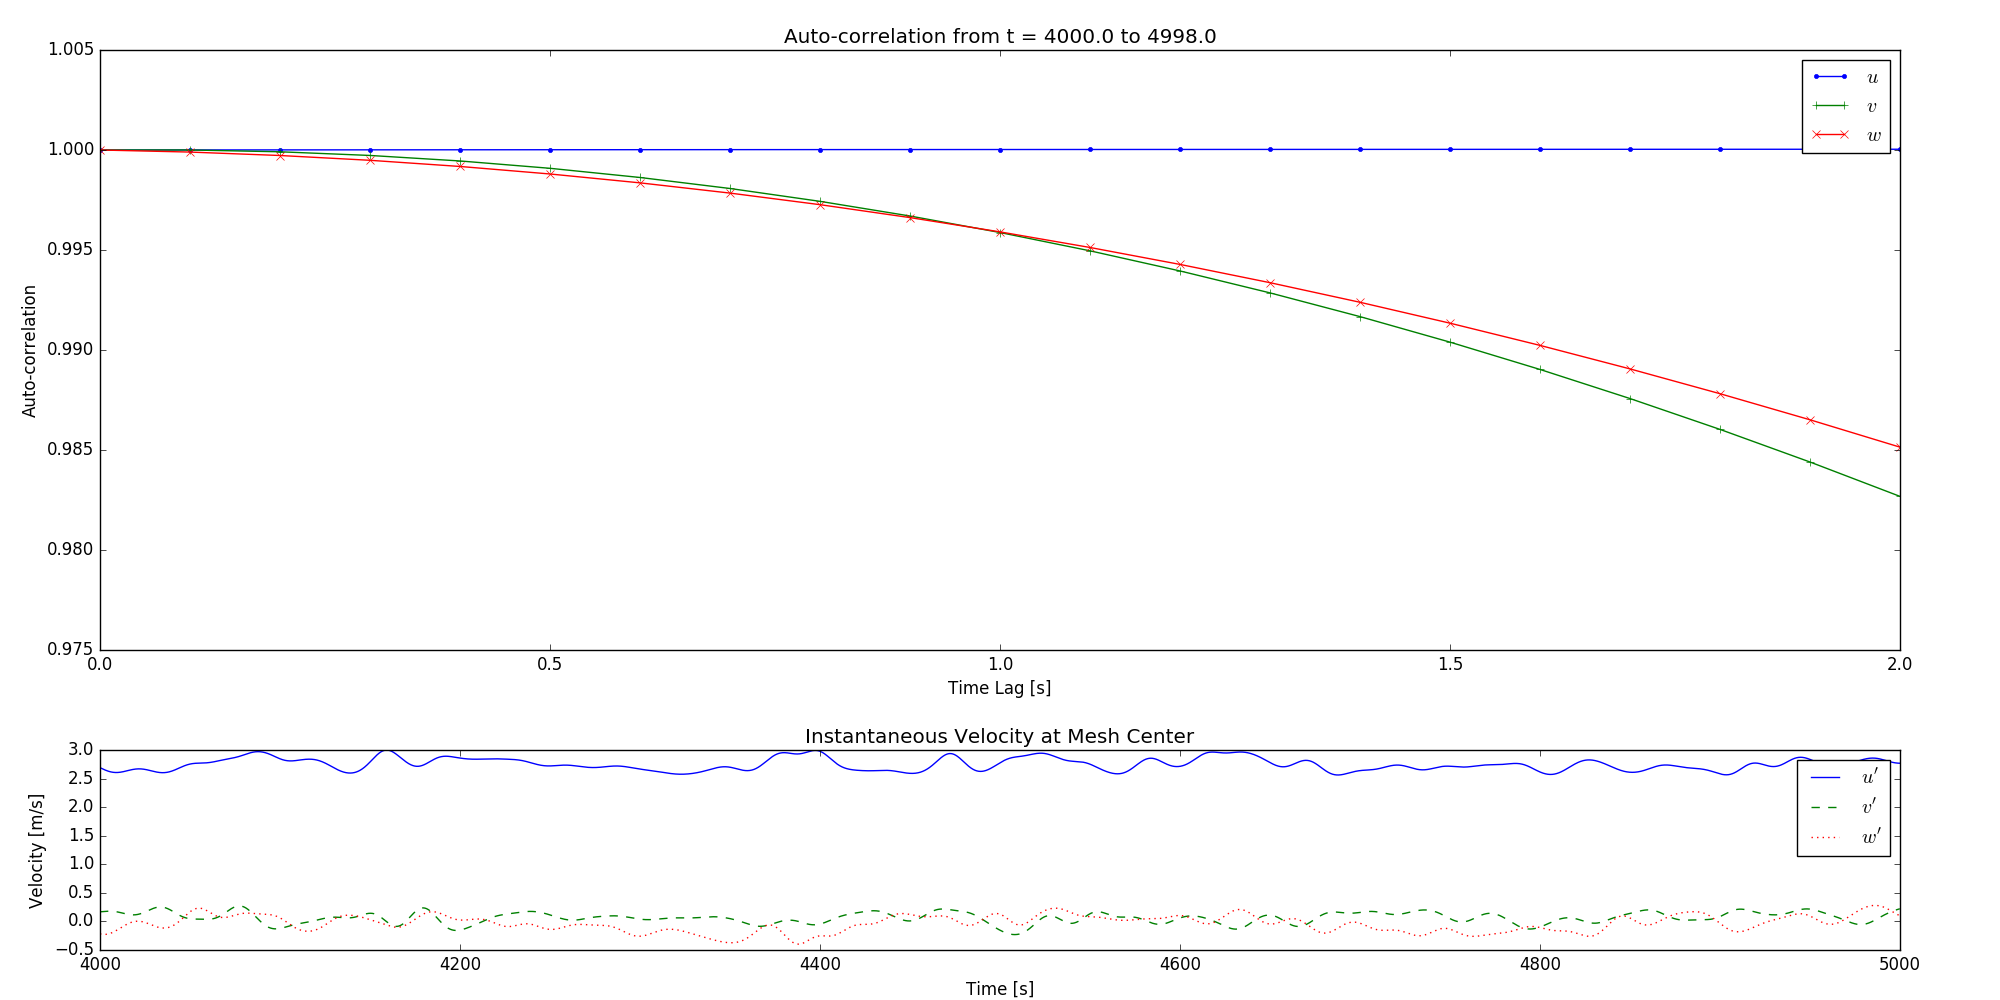
\includegraphics[scale=0.35]{nutU/keq_stability.png}
\caption{Auto-correlation of each velocity component with increased time lag (above) and instantaneous values of velocity components (below) for the One-Equation Eddy Viscosity SGS, using the \texttt{nutUWallFunction}.}
\label{nutU_keq_stab}
\end{figure}
  
\begin{figure}[H]
\centering
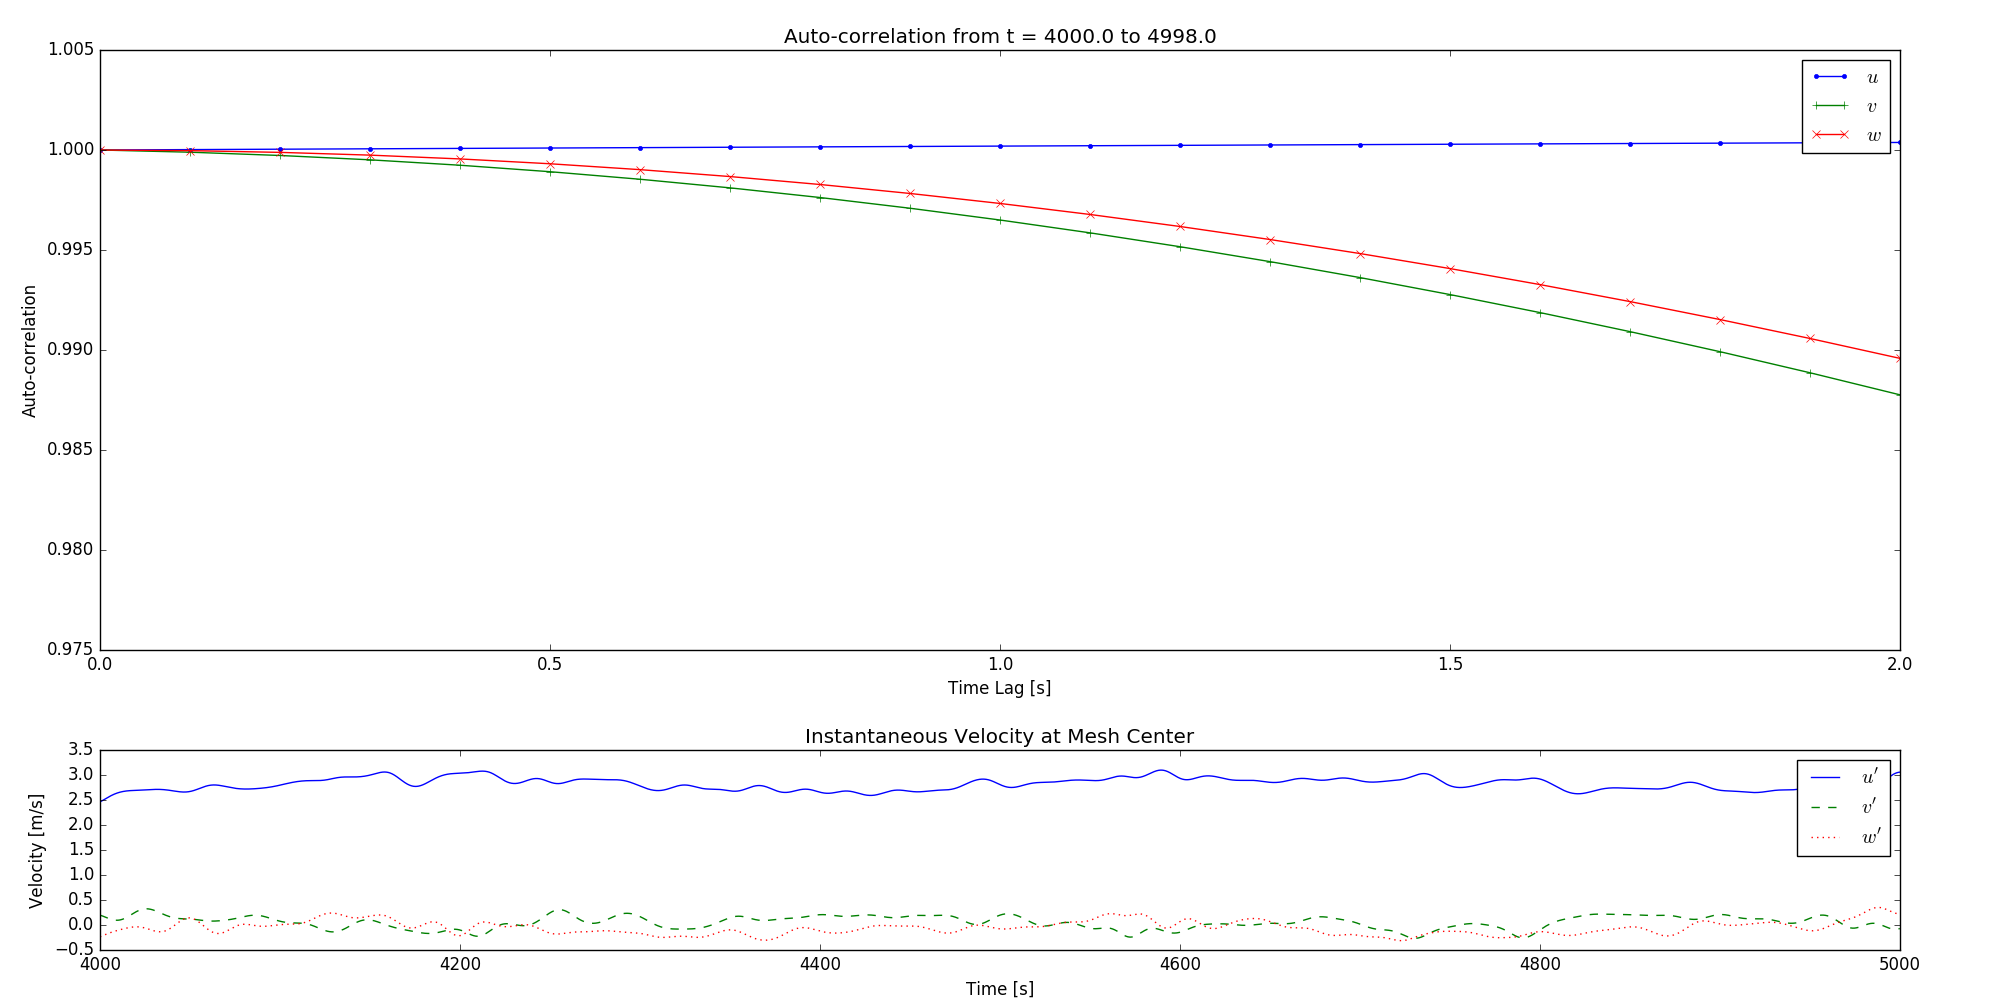
\includegraphics[scale=0.35]{nutU/sm_stability.png}
\caption{Auto-correlation of each velocity component with increased time lag (above) and instantaneous values of velocity components (below) for the Smagorinsky SGS, using the \texttt{nutUWallFunction}.}
\label{nutU_sm_stab}
\end{figure}

\begin{figure}[H]
\centering
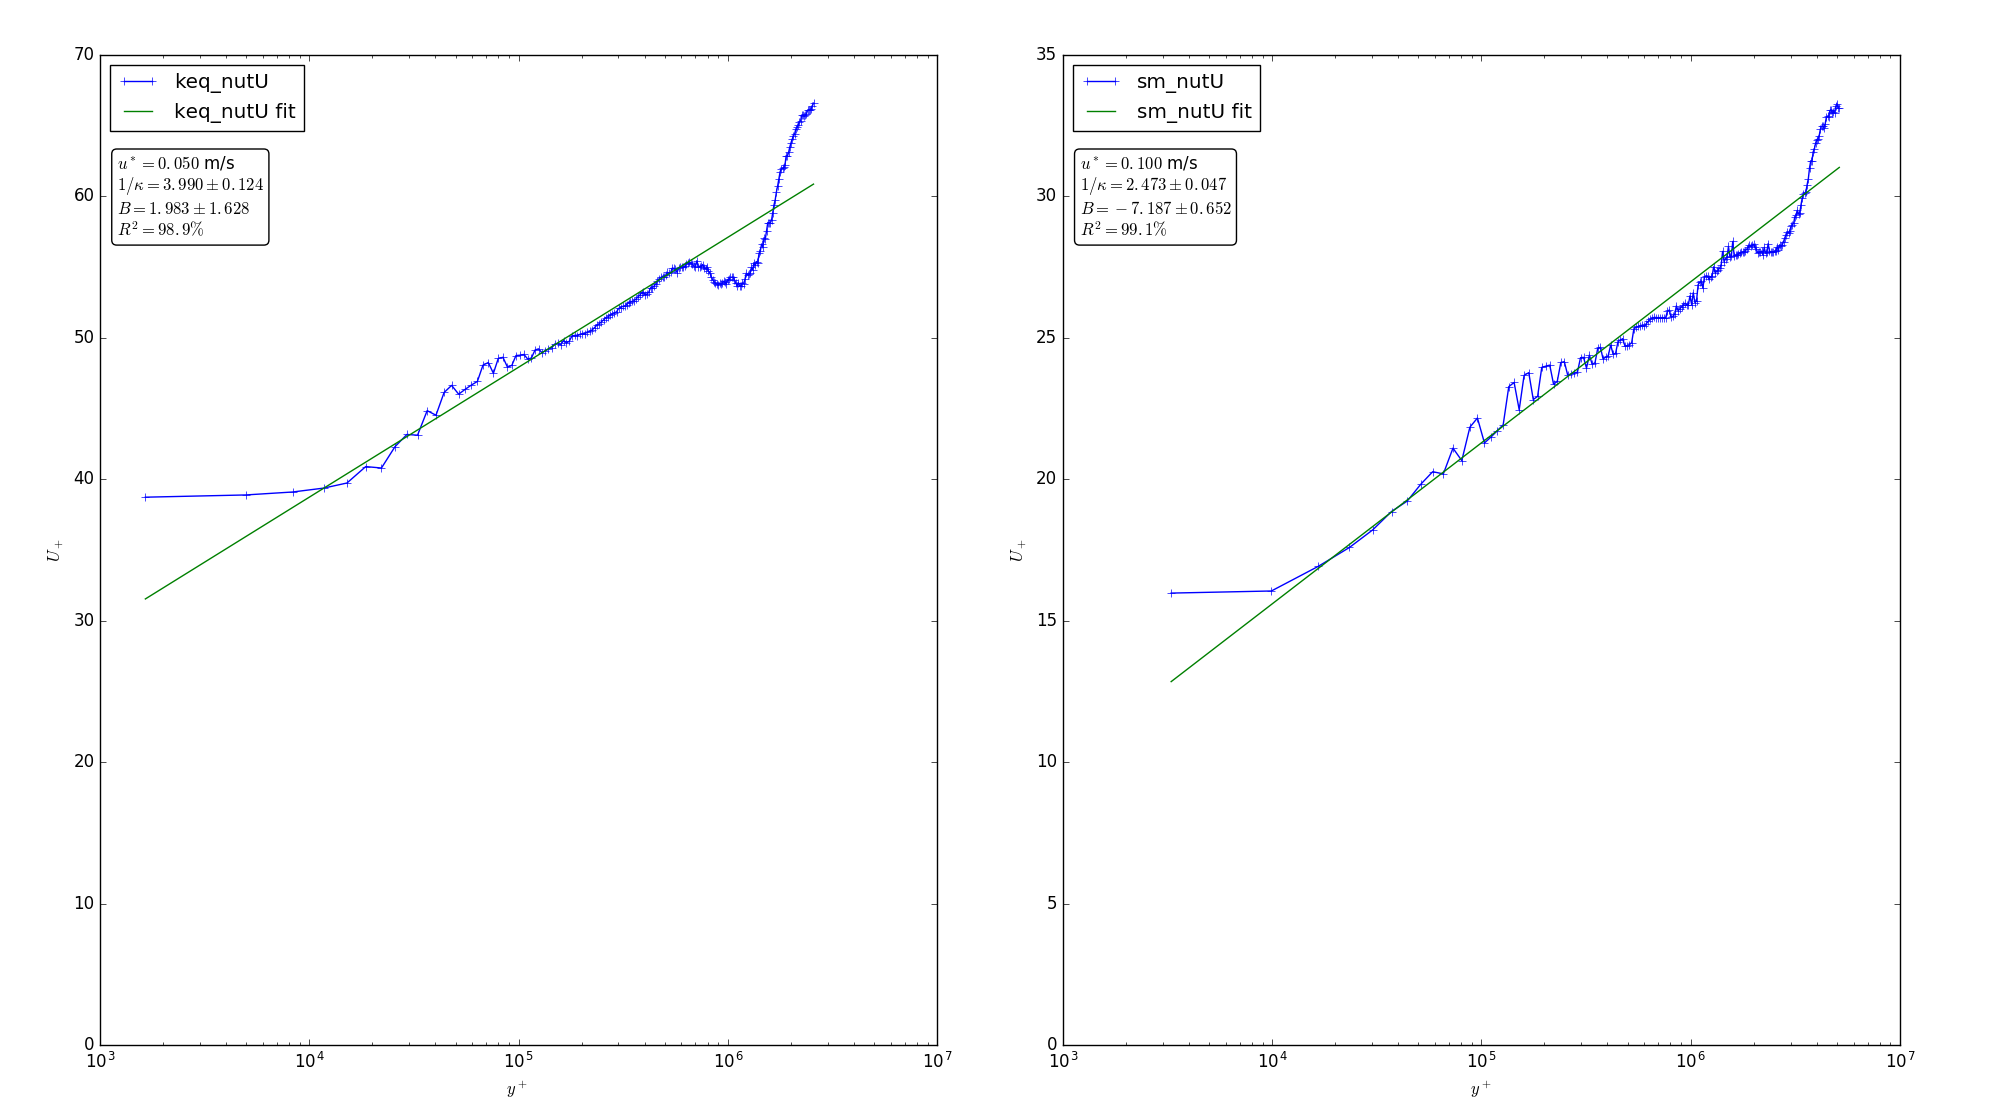
\includegraphics[scale=0.35]{nutU/keq_sm_log.png}
\caption{Log-linear fit of the mean vertical velocity profile for the One-Equation Eddy Viscosity (left) and the Smagorinsky (right) SGS models, using the \texttt{nutUWallFunction}.}
\label{nutU_keq_sm_log}
\end{figure}

\pagebreak
\bibliography{references.bib}

\end{document}